\documentclass[10pt,a4paper,twoside]{article}
\usepackage[utf8]{inputenc}
\usepackage{fancyhdr}
\usepackage[english,german]{babel}
\usepackage[margin=1in,inner=1.2in]{geometry}
\usepackage[parfill]{parskip}
\usepackage{makeidx}
\usepackage[onehalfspacing]{setspace}
\usepackage{fancyhdr}
\usepackage{lastpage}
\usepackage{hyperref}
\usepackage{multicol}
\usepackage{graphicx}
\renewcommand{\familydefault}{ptm}

\title{\textbf{Physik}\\Notizen für Prüfung vom 1. März 2016}
\author{Patrick Günthard}

\pagestyle{fancy}
\fancyhf{}
\fancyhead[EL]{Notizen Prüfung}
\fancyhead[OR]{Patrick Günthard}
\cfoot{\thepage \space von \pageref{LastPage}}

\begin{document}
	\maketitle
	\tableofcontents
	
	\clearpage
	
	\section{Horizontaler Wurf}
	\textit{Alle Formeln gelten nur für Berechnungen im Vakuum, daher gilt für \(v\) (wenn ohne einfluss von \(a\)) \(v_n = v_0\) und \(a_n = a_0\)}
	\subsection{Formeln}
	\subsubsection{x-Richtung}
	\begin{multicols}{2}
		\(s_x = v_0t ( = v_nt)\)\\
		\(v_x = v_0\)\\
		\(a_x = 0\)
	\end{multicols}
	\subsubsection{y-Richtung}
	\begin{multicols}{2}
		\textbf{Standardberechnungen:}\\
		
		\(s_y = - \frac{gt^2}{2} - h_0\) \footnote{\(h_0 = s_{y0}\)}  \\
		\(v_y = gt\) \footnote{\(g \approx 9.81\) auf der Erde, Messung von Potsdam (BRD). An anderen Orten wurde \(g = \approx 9.79\) gemessen. Für unsere Berechnungen ist der erstgenannte Messwert relevant da er geographisch am nächsten liegt.}
		\(a_y = g\) 
		
		\textbf{Berechnungen Parabel:}\\
		
		\(s_y = -\frac{g}{2}(\frac{s_x}{v_0})^2 + h_0\) \textit{(Bei dieser Formel wird \(t\) aufgelöst)} (\(t = (\frac{s_x}{v_0})^2\))
		
	\end{multicols}
	
	\subsubsection{Weitere Berechnungen}
	
	\begin{multicols}{2}
		\textit{Wurfweite:} \(s_w = v_0 \sqrt{ \frac{2h_0}{g} } \)\\
		\textit{Wurfhöhe:}  \(s_h = \frac{gs_w^2}{2v_0^2}\)\\
		\textit{Wurfdauer:} \(t_w = \sqrt{ \frac{2h_0}{g} }\)
	\end{multicols}
	
	\subsubsection{Parabel}
	
	\begin{multicols}{2}
		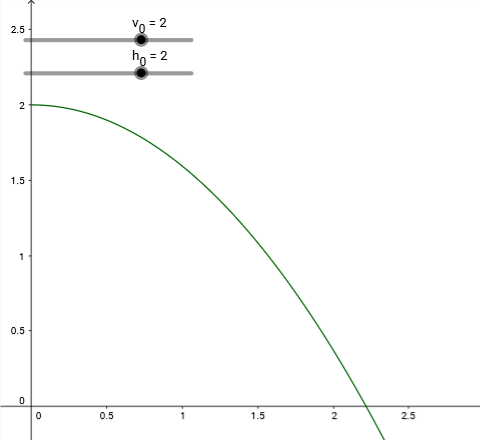
\includegraphics[width=6cm]{img/wurf_example}\\
		
		\textbf{Bei der Parabel wurden folgende Parameter verwendet:}\\
		\(v_0 = 2\frac{m}{s}\)\\
		\(h_0 = h_{y0} = 2m\)\\
		\(g = 9.81\)
	\end{multicols}
	\section{Dynamik}
	
	In der Dynamik wird mit \textit{Kräften} (\(F\))\footnote{Die Abkürzung \(F\) kommt von \textit{force}, dem englischen Wort für \textit{Kraft}} gerechnet. Es gibt verschiedene Kräfte welche (auf der Erde) \textbf{immer} wirken:
	
	\begin{itemize}
		\item Die \textit{Normalkraft}: \(\vec{F_N}\)
		\item Die \textit{Gewichtskraft}: \(\vec{F_G} = m * \vec{g}\)
	\end{itemize}
	
	
	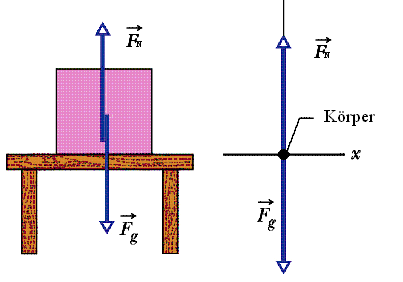
\includegraphics[width=5cm]{img/force_example}\\
	Wenn ein Körper stillsteht, heben sich beide Kräfte auf: \( \vec{F_N} = - \vec{F_G}\)
	
	\subsection{Formeln}

	\subsubsection{Basisformeln}
	
	\begin{multicols}{2}
		\(\vec{F} = m * \vec{a}\) \footnote{Wobei \(-a = g\)} \\
		\(F\) ist dabei \textit{Kraft} welche in \textit{Newton} \footnote{Benannt nach \textit{Isaac Newton} (1643 - 1727), Englischer Physiker} (\(N\)) gemessen wird. Ein Beispiel wie \(N\) berechnet wird:\\
		\(1N = 1kg * \frac{m}{s^2}\)
		
	\end{multicols}
	
\end{document}